\documentclass[11pt, addpoints, answers]{exam}

\usepackage[utf8]{inputenc}
\usepackage[T1]{fontenc}
\usepackage[margin  = 1in]{geometry}
\usepackage{amsmath, amscd, amssymb, amsthm, verbatim}
\usepackage{mathabx}
\usepackage{setspace}
\usepackage{float}
\usepackage{color}
\usepackage{graphicx}
\usepackage[colorlinks=true]{hyperref}
\usepackage{tikz}

\usetikzlibrary{shapes,arrows}
%%%<
\usepackage{verbatim}
%%%>
\usetikzlibrary{automata,arrows,positioning,calc}

\usetikzlibrary{trees}

\shadedsolutions
\definecolor{SolutionColor}{RGB}{214,240,234}

\newcommand{\bbC}{{\mathbb C}}
\newcommand{\R}{\mathbb{R}}            % real numbers
\newcommand{\bbR}{{\mathbb R}}
\newcommand{\Z}{\mathbb{Z}}            % integers
\newcommand{\bbZ}{{\mathbb Z}}
\newcommand{\bx}{\mathbf x}            % boldface x
\newcommand{\by}{\mathbf y}            % boldface y
\newcommand{\bz}{\mathbf z}            % boldface z
\newcommand{\bn}{\mathbf n}            % boldface n
\newcommand{\br}{\mathbf r}            % boldface r
\newcommand{\bc}{\mathbf c}            % boldface c
\newcommand{\be}{\mathbf e}            % boldface e
\newcommand{\bE}{\mathbb E}            % blackboard E
\newcommand{\bP}{\mathbb P}            % blackboard P

\newcommand{\ve}{\varepsilon}          % varepsilon
\newcommand{\avg}[1]{\left< #1 \right>} % for average
%\renewcommand{\vec}[1]{\mathbf{#1}} % bold vectors
\newcommand{\grad}{\nabla }
\newcommand{\lb}{\langle }
\newcommand{\rb}{\rangle }

\def\Bin{\operatorname{Bin}}
\def\Var{\operatorname{Var}}
\def\Geom{\operatorname{Geom}}
\def\Pois{\operatorname{Pois}}
\def\Exp{\operatorname{Exp}}
\newcommand{\Ber}{\operatorname{Ber}}
\def\Unif{\operatorname{Unif}}
\def\No{\operatorname{N}}
\newcommand{\E}{\mathbb E}            % blackboard E
\def\th{\theta }            % theta shortcut
\def\V{\operatorname{Var}}
\def\Var{\operatorname{Var}}
\def\Cov{\operatorname{Cov}}
\def\Corr{\operatorname{Corr}}
\newcommand{\epsi}{\varepsilon}            % epsilon shortcut

\providecommand{\norm}[1]{\left\lVert#1\right\rVert} %norm
\providecommand{\abs}[1]{\left \lvert#1\right \rvert} %absolute value

\DeclareMathOperator{\lcm}{lcm}
\newcommand{\ds}{\displaystyle}	% displaystyle shortcut

\def\semester{2019-2020}
\def\course{Modèles Aléatoires Discrets}
\def\title{\MakeUppercase{Examen Final}}
\def\name{Pierre-O Goffard}
%\def\name{Professor Wildman}

\setlength\parindent{0pt}

\cellwidth{.35in} %sets the minimum width of the blank cells to length
\gradetablestretch{2.5}

%\bracketedpoints
%\pointsinmargin
%\pointsinrightmargin

\begin{document}


\runningheader{\course  \vspace*{.25in}}{}{\title \vspace*{.25in}}
%\runningheadrule
\runningfooter{}{Page \thepage\ of \numpages}{}

% \firstpageheader{Name:\enspace\hbox to 2.5in{\hrulefill}\\  \vspace*{2em} Section: (circle one) TR: 3-3:50 \textbar\, TR: 5-5:50 \textbar\,  TR: 6-6:50(Xu) \textbar\,  TR: 6-6:50 }{}{Perm \#: \enspace\hbox to 1.5in{\hrulefill}\\ \vspace*{2em} Score:\enspace\hbox to .6in{\hrulefill} $/$\numpoints}
\extraheadheight{.25in}

\hrulefill

\vspace*{1em}

% Heading
{\center \textsc{\Large\title}\\
	\vspace*{1em}
	\course -- \semester\\
	Pierre-O Goffard\\
}
\vspace*{1em}

\hrulefill

\vspace*{2em}

\noindent {\bf\em Instructions:} On éteint et on range son téléphone.
\begin{itemize}
	\item La calculatrice et les appareils éléctroniques ne sont pas autorisés.
	\item Vous devez justifier vos réponses de manière claire et concise.
	\item Vous devez écrire de la manière la plus lisible possible. Souligner ou encadrer votre réponse finale.

\end{itemize}

\begin{center}
	\gradetable[h]
\end{center}

\smallskip

\begin{questions}
\question Questions de cours. Processus de Poisson. 
\begin{parts}
\part[1] Soit $X\sim \text{Exp}(\lambda)$, montrer que 
$$
\mathbb{P}(X>t+s|X>t)=\mathbb{P}(X>s),\text{ }s,t>0.
$$  
\part[1] Rappeler la définition d'un processus de Poisson $(N_t)_{t\geq0}$
\part[1] Soit $(N_t)_{t\geq0}$ un processus de Poisson, montrer que 
$$
\mathbb{P}(N_t = k)=\frac{e^{-\lambda}\lambda^k}{k!},\text{ }k\geq0.
$$
\begin{solution}
Voir le cours.
\end{solution}
\end{parts}
\question On suppose qu'une playlist (pour aller courir) contient $3$ chansons différentes. On définit le processus $(X_n)_{n\in\mathbb{N}}$ égale au nombre de chansons différentes écoutées jusqu'à l'instant $n\in\mathbb{N}$. On suppose que $X_0=0$.
\begin{parts}
\part[1] Le processus $(X_n)_{n\in\mathbb{N}}$ définit une chaine de Markov homogène. Donner son espace d'état, sa loi initiale, sa matrice des transitions et son graphe des transitions.
\begin{solution}
$E = \{0,1,2,3\}$, $\mu = (1,0,0,0)$, La matrice des transitions est données par 
$$
Q =\left(\begin{array}{cccc}
0&1&0&0\\
0&1/3&2/3&0\\
0&0&2/3&1/3\\
0&0&0&1\\
\end{array}\right)
$$
et le graph des transition
\begin{center}
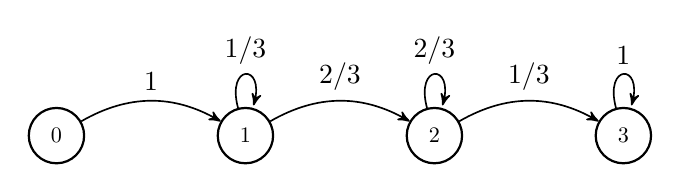
\begin{tikzpicture}[->, >=stealth', auto, semithick, node distance=3cm]
\tikzstyle{every state}=[fill=white,draw=black,thick,text=black,scale=0.8]
\node[state]    (1)                     {$0$};
\node[state]    (2)[right of=1]   {$1$};
\node[state]    (3)[right of=2]   {$2$};
\node[state]    (4)[right of=3]   {$3$};
\path
(1) edge[bend left]     node{$1$}         (2)

(2) edge[loop above]      node{$1/3$}      (2)
    edge[bend left]     node{$2/3$}      (3)
(3) edge[loop above]      node{$2/3$}      (3)
    edge[bend left]     node{$1/3$}      (4)
(4) edge[loop above]      node{$1$}     (4);


\end{tikzpicture}
\end{center}
\end{solution}
\part[1] $(X_n)_{n\in\mathbb{N}}$ est elle irréductible? Justifier.
\begin{solution}
L'espace d'état comprend $4$ classes de communications dont 
\begin{itemize}
  \item $\{0\}$, $\{1\}$, et $\{2\}$ sont des classes ouvertes
  \item $\{3\}$ est une classe fermée. 
\end{itemize}
La chaine n'est donc pas irréductible.
\end{solution}
\part[2] Discuter l'existence et l'unicité d'une loi stationnaire.
\begin{solution}
L'espace d'état est fini, il existe au moins une loi stationnaire. Celle ci est unique car on n'a qu'une seule classe fermée, la loi stationnaire est donnée par $\pi=(0,0,0,1)$
\end{solution}
\part[1] On note $\tau_{3} = \inf\{n\geq0\text{ ; }X_n = 3\}$. $\tau_3$ est-il un temps d'arrêt? Justifier.
\begin{solution}
On peut écrire 
$$
\{\tau_{3} = n\} = \bigcap_{k = 0}^{n-1}\{X_k \neq 3\}\cap\{X_n = 3\} \in \mathcal{F}_n,
$$
avec $\mathcal{F}_n = \sigma(X_0,\ldots,X_n)$. 

\end{solution}
\part[2] En utilisant une analyse à un pas, donner $\E_0(\tau_3):=\E(\tau_3|X_
0=0)$.
\begin{solution}
On résout le système suivant 
\begin{eqnarray}
\E_0(\tau_3)&=&1 + \E_1(\tau_3)\label{eq1} \\
\E_1(\tau_3)&=&1 + \E_1(\tau_3)/3 + 2\E_2(\tau_3)/3\label{eq2} \\
\E_2(\tau_3)&=&1 + 2\E_2(\tau_3)/3 \label{eq3} 
\end{eqnarray}
On obtient $\E_2(\tau_3)=3$, $\E_1(\tau_3)=9/2$ et $\E_0(\tau_3)=11/2.$

\end{solution}
\end{parts}
\question La vie de Pierre-O. \\

Nous allons géolocaliser Pierre-O heure par heure à l'aide d'une chaine de Markov homogène $(X_n)_{n\geq0}$. Pierre-O peut se trouver dans $3$ positions
\begin{enumerate}
  \item Maison
  \item ISFA
  \item Bar
\end{enumerate}
On suppose qu'initialement il peut se trouver dans un de ces trois endroits de manière equiprobable. Ensuite ses déplacements suivent la dynamique suivante 
\begin{itemize}
  \item lorsqu'il est à la maison il peut rester à la maison, aller à l'ISFA ou aller ou bar de manière equiprobable
  \item lorsqu'il est à l'ISFA il va au bar dans $50\%$ des cas, va à la maison dans $25\%$ des cas, reste à l'ISFA dans $25\%$ des cas
  \item lorsqu'il est au bar soit il reste au bar, soit il rentre à la maison de manière équiprobable.
\end{itemize}
\begin{parts}
\part[1] Donner l'espace d'état, la loi initiale, le graph des transitions et la matrice des transitions de $(X_n)_{n\in\mathbb{N}}$.
\begin{solution}
L'espace d'état est donné par $E = \{1,2,3\}$, la loi initiale est $\mu = \left(1/3,1/3,1/3\right)$. Le graph des transitions est le suivant
\begin{center}
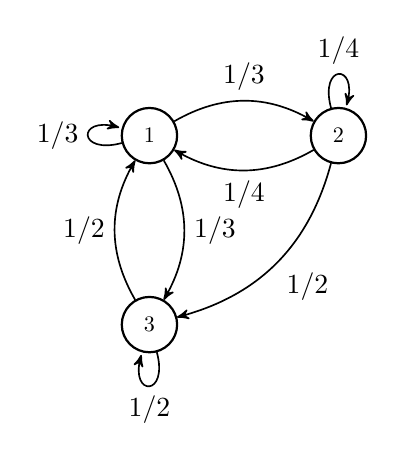
\begin{tikzpicture}[->, >=stealth', auto, semithick, node distance=3cm]
\tikzstyle{every state}=[fill=white,draw=black,thick,text=black,scale=0.8]
\node[state]    (1)               {$1$};
\node[state]    (2)[right of=1]   {$2$};
\node[state]    (3)[below of=1]   {$3$};
\path
(1) edge[bend left]     node{$1/3$}        (2)
(1) edge[bend left]     node{$1/3$}        (3)
(1) edge[loop left]     node{$1/3$}        (1)

(2) edge[loop above]      node{$1/4$}    (2)
    edge[bend left]     node{$1/2$}      (3)
    edge[bend left]     node{$1/4$}      (1)
(3) edge[loop below]      node{$1/2$}    (3)
(3) edge[bend left]      node{$1/2$}    (1);

\end{tikzpicture}
\end{center}
La matrice des transition est donnée par 
$$
Q =\left(\begin{array}{ccc}
1/3&1/3&1/3\\
1/4&1/4&1/2\\
1/2&0&1/2
\end{array}\right)
$$

\end{solution}
\part[1] La chaine est-elle irréductible?
\begin{solution}
Oui, il n'y a qu'une seule classe de communication
\end{solution}  
\part[1] Donner la période de chaque état
\begin{solution}
Tous les états sont dans la même classe de communication et ont donc même période, celle ci est égale à 1 car par exemple
$$
d(1) =\text{pgcd}\{1,2,\ldots\} = 1
$$
\end{solution}
\part[2] Après avoir justifié son existence et son unicité, donner la loi stationnaire de $(X_n)_{n\in\mathbb{N}}$.
\begin{solution}
L'espace d'état est de dimension fini, la loi stationnaire existe. Comme la chaine est irréductible alors la loi stationaire est unique et solution de 
$$\begin{cases}
\pi.Q = \pi&\\
\pi.\mathbf{1}_3 = 1& 
\end{cases}$$
On trouve $\pi = (9/23,4/23, 10/23)$
\end{solution} 
\end{parts}

\question L'objectif est de modéliser le temps d'attente à un guichet d'un guichet ouvert 24 heures sur 24. Les clients arrivent au guichet suivant un processus de Poisson $(N_t)_{t\geq0}$ d'intensité $\lambda$, l'unité de temps est l'heure. Le temps de service pour chaque client est une variable aléatoire $X$, positive, continue (à densité par rapport à la mesure de Lebesgue). Le temps d'occupation effectif du guichet est donné par un processus de Poisson composé défini par 
$$
S_t = \sum_{i=1}^{N_t} X_i,\text{ }t\geq0.
$$ 
où $(X_i)_{i\geq1}$ est une suite i.i.d. de variables aléatoires distribuées comme $X$, indépendantes de $(N_t)_{t\geq0}$. Le temps d'attente d'un client arrivant à l'instant $t$ est un processus donné par 
$$
R_t = \left(S_t - t\right)_+,\text{ }t\geq0
$$
où $(x)_+ = \max(x,0),\text{ }x\in \mathbb{R}$ désigne la fonction partie positive.
\begin{parts}
  \part[1] Lors de la première journée qui démarre à $0:00$ heure, quelle est la probabilité d'avoir entre $2$ et $4$ clients entre $8:00$ et $11:00$. Donner le résultat en fonction de $\lambda$.
  \begin{solution}
  On calcule 
  \begin{eqnarray*}
  \mathbb{P}(N_11-N_8\in \{2,3,4\}) &=&\mathbb{P}(N_3= 2)+\mathbb{P}(N_3= 3)+\mathbb{P}(N_3= 4)\\
  &=&\frac{e^{-3\lambda}(3\lambda)^2}{2!}+\frac{e^{-3\lambda}(3\lambda)^3}{3!}+ \frac{e^{-3\lambda}(3\lambda)^4}{4!}
  \end{eqnarray*}
  \end{solution}
  \part[2] Le temps de traitement de la demande d'un client suit une loi de Weibull $X\sim \text{Weibull}(\alpha,\beta)$ de densité (par rapport à la mesure de Lebesgue) donnée par 
  $$
  f_X(x) = \left(\frac{\alpha}{\beta}\right)\left(\frac{x}{\beta}\right)^{\alpha-1}\exp\left(-\left(\frac{x}{\beta}\right)^\alpha\right),\text{ }x>0,\text{ }\alpha,\beta>0.
  $$
  Calculer $\E(X^k)$ pour $k\geq1$. Donner le résultat en fonction de $\alpha$, $\beta$ et de la fonction gamma définie par 
  $$
  \Gamma(z) = \int_{0}^{+\infty}x^{z-1}e^{-x}\text{d}x,\text{ avec }z>0.
  $$
  \begin{solution}
  On a 
  \begin{eqnarray*}
  \E(X^k) &=& \int_{0}^{+\infty}x^k\left(\frac{\alpha}{\beta}\right)\left(\frac{x}{\beta}\right)^{\alpha-1}\exp\left(-\left(\frac{x}{\beta}\right)^\alpha\right)\text{d}x\\
  &=&\int_{0}^{+\infty}\beta^k y^{k/\alpha}e^{-y}\text{d}y\\
  &=&\beta^k\Gamma\left(1+k/\alpha\right)
  \end{eqnarray*}
  \end{solution}
  \part[1] Donner la moyenne et la variance de $S_t$ pour un instant $t>0$ en fonction de $\alpha$, $\beta$ et $\lambda$. Si vous n'êtes pas parvenu à résoudre la question précédente, vous pouvez noter $\mu = \E(X)$ et $\sigma^2 = \text{Var}(X)$.
  \begin{solution}
  On a 
  $$
\E(S_t)=\E(N)\E(X)=\lambda t\beta\Gamma(1+1/\alpha)
  $$
  et 
  $$
  \V(S_t)=t\lambda\beta^2\Gamma(1+2/\alpha)
  $$
  \end{solution}
  \part[1] On approche la distribution de $(S_t)_{t\geq0}$ (approximation grossière) par une loi exponentielle de paramètre $1/\E(S_t)$ (L'atome de probabilité en $0$ de $S_t$ peut en particulier être négligé pour $\lambda$ grand). En utilisant cette approximation, donner l'expression du temps d'attente moyen $\mathbb{E}(R_t)$ à l'instant $t\geq0$ en fonction de $\lambda, t, \alpha$, et $\beta$ (à défaut $\mu$ si vous n'êtes pas parvenu à répondre à la question b).  
  \begin{solution}
  On a 
  \begin{eqnarray*}
  \mathbb{E}\left[(S_t-t)_+\right]&=&\mathbb{E}\left[(S_t-t)\mathbb{I}_{S_t>t}\right]\\
  &=&\mathbb{E}\left(S_t\mathbb{I}_{S_t>t}\right)-t\mathbb{P}\left(S_t>t\right)\\
  &=& \lambda t\beta\Gamma(1+1/\alpha) \exp\left(-1/\lambda \beta\Gamma(1+1/\alpha)\right)
  \end{eqnarray*}
  \end{solution}
\end{parts} 
\end{questions}
%-------------------------------TABLE-------------------------------
\newpage
\hrule
\vspace*{.15in}
\begin{center}
  \large\MakeUppercase{Formulaire}
\end{center}
\vspace*{.15in}
\hrule
\vspace*{.25in}

\renewcommand\arraystretch{3.5}
\begin{table}[H]
\begin{center}
\footnotesize
\begin{tabular}{|c|c|c|c|c|c|}

\hline
Nom & abbrev. & Loi & $\E(X)$ & $\Var(X)$ & FGM\\
\hline\hline
Binomial & $\Bin(n,p)$ & $\binom{n}{k}p^k(1-p)^{n-k}$ & $np$ & $np(1-p)$ & $[(1-p)+pe^t]^n$\\
\hline
Poisson & $\Pois(\lambda)$ & $e^{-\lambda}\dfrac{\lambda^k}{k!}$ & $\lambda$ & $\lambda$ &$ \exp(\lambda(e^t-1))$\\
\hline
Geometric & $\Geom(p)$ & $(1-p)^{k-1}p$ & $\dfrac{1}{p}$ & $\dfrac{1-p}{p^2}$ & $\frac{pe^t}{1-(1-p)e^t}$ pour  $t<-\ln(1-p)$\\
\hline
Uniform & $\Unif(a,b)$ & $\begin{cases} \dfrac{1}{b-a} & a\leq t\leq b\\ 0 & \text{sinon}\end{cases}
$ & $\dfrac{a+b}{2}$ & $\dfrac{(b-a)^2}{12}$ & $\frac{e^{tb}-e^{ta}}{t(b-a)}$\\
\hline
Exponential & $\Exp(\lambda)$ & $\begin{cases} \lambda e^{-\lambda t} & t\geq 0 \\ 0 & t<0\end{cases}$ & $\dfrac{1}{\lambda}$ & $\dfrac{1}{\lambda^2}$ & $\frac{\lambda}{\lambda -t}$ pour $t<\lambda$\\
\hline
Normal & $\No(\mu,\sigma^2)$ & $\left(\dfrac{1}{\sqrt{2\pi\sigma^2}}\right)\operatorname{exp}{\left(\dfrac{-(t-\mu)^2}{2\sigma^2}\right)}$ & $\mu$ & $\sigma^2$ & $e^{\mu t}e^{\sigma^2t^2/2}$\\
\hline
\end{tabular}
\end{center}
\end{table}%

\end{document}